\header{
    \section{Trent'six matelots} \label{trent-six-matelots}
    %
    
    \insertComment{}{}
}

\enluminure{2}{\href{}{J}}{e vois} venir la barque
\\De trent'six matelots !
\dualcol{
\\\\De trent'six matelots
\\Sur le bord de la France
\\De trent'six matelots
\\Sur le bord de l'eau
\\Tout auprès du vaisseau
\\\\Le plus jeune des trente
\\Commence une chanson
\\\\Commence une chanson
\\Sur le bord de la France
\\Commence une chanson
\\Sur le bord de l'eau
\\Tout auprès du vaisseau
\\\\\textbf{Sur la même construction :}
\\\\La chanson que tu chantes
\\J'voudrais bien la savoir !
\\\\Bell' rentrez dans la barque
\\Bell' je vous l'apprendrai
\\\\Quand la belle fut dans la barque,
\\Elle s'est endormie.
\\\\Quand la belle s'éveille
\\Elle se mit à pleurer
\\\\Que pleurez vous la belle
\\Qu'avez vous à pleurer ?
\\\\Je pleure mon coeur en gage,
\\Galant que vous avez !
\\\\Ne pleurez pas la belle
\\Vot' coeur je vous l'rendrai !
\bigskip
\begin{center}
\centering
    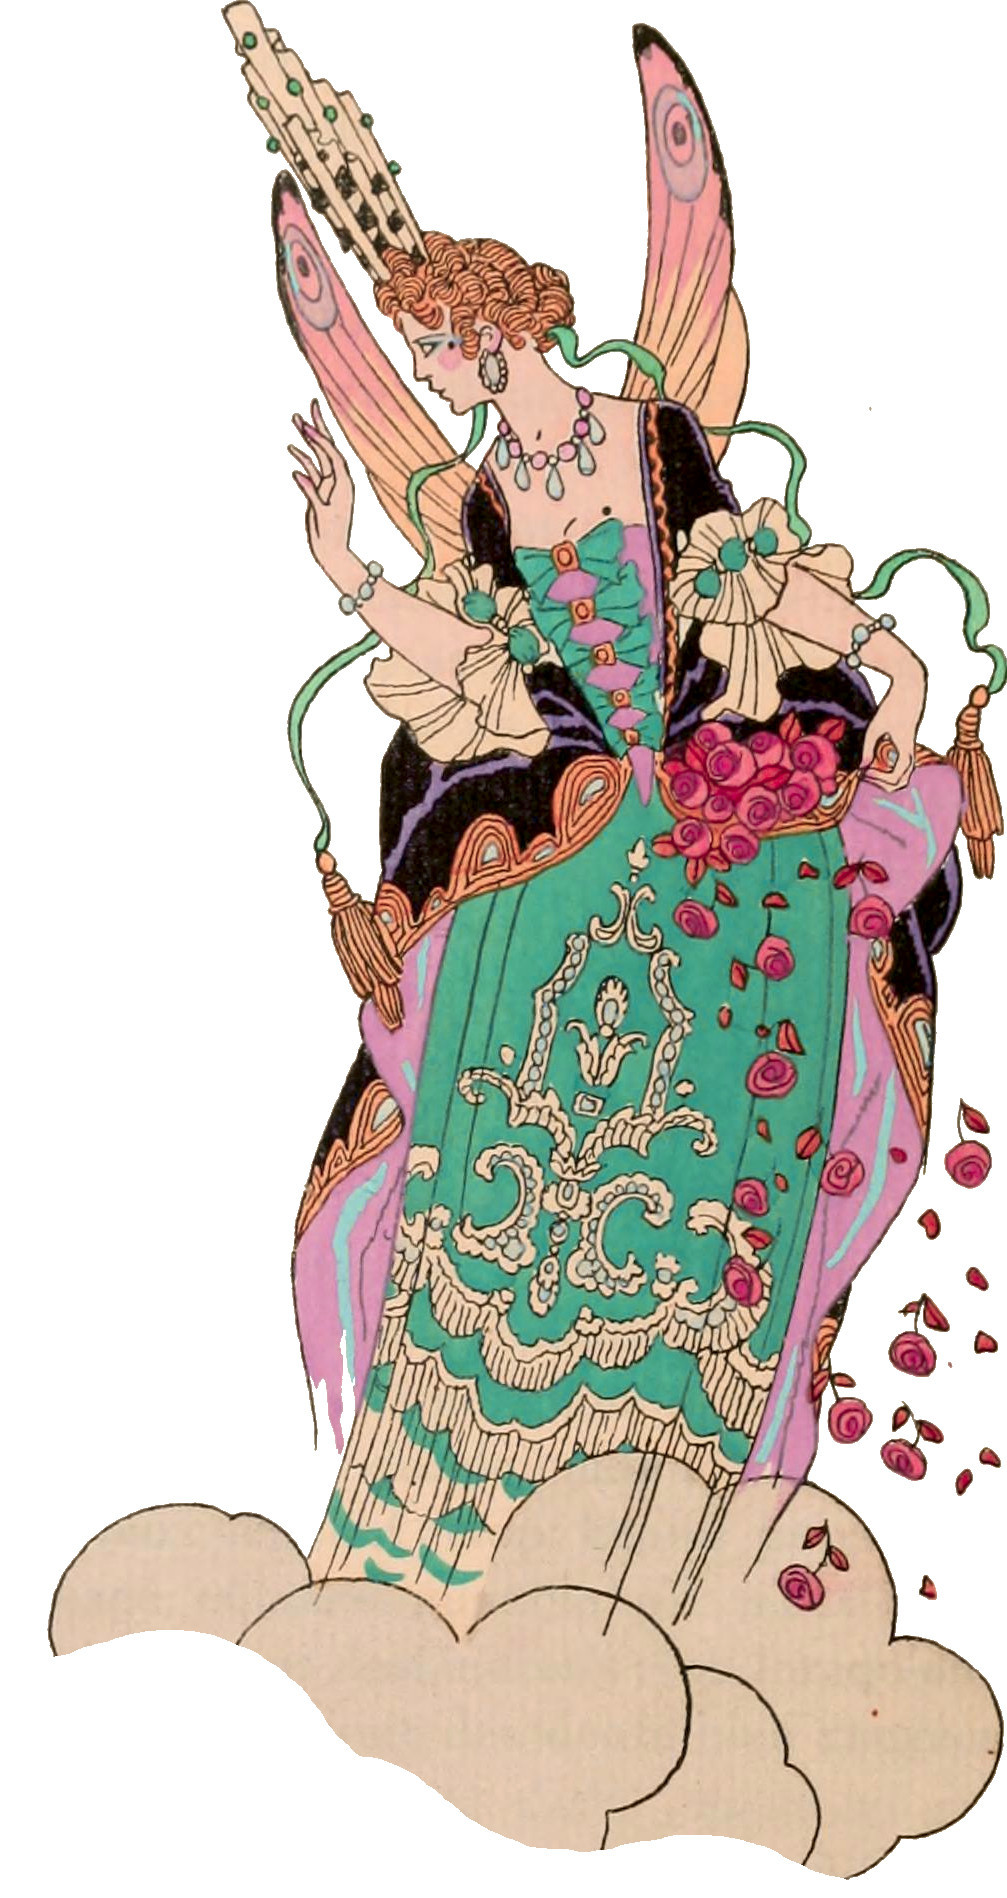
\includegraphics[width=0.5\textwidth]{images/brev48.png}
 \end{center}
}
 
\breakpage